\documentclass[a4paper,11pt]{article}
\usepackage{fancyhdr}
\usepackage[utf8]{inputenc}
\usepackage{graphicx}
%\setlength{\headheight}{11pt}

\lhead
\rhead
\parskip 1em
\parindent 0em

\begin{document}
\pagestyle{empty}
%-----------------------------------------------------------
\begin{titlepage}

\title{\Huge{Lab report} \\[0.1cm] \Large{Digital Design (EDA322)} \\ [0.4cm] \Large{ \emph{Writing Guidelines}} \\[0.4cm]}
\author{\large{\emph{Group TUE\_PM\_8}} \\[0.2cm] Niklas Gustafsson \\[0.05cm] Oskar Lundström \\[0.1cm]}
\maketitle
\thispagestyle{empty}
\end{titlepage}
\clearpage
%-----------------------------------------------------------
\pagestyle{fancyplain}
\pagenumbering{roman}
\tableofcontents
\clearpage
%%%%%%%%%%%%%%%%
% Introduction
\pagenumbering{arabic}
\setcounter{page}{1}
\section{Introduction}
(max: 1 page)
\\\\
This part will introduce the reader to the report. 

At the beginning, describe what the purpose of this lab report is. Then describe briefly what each section discusses and finally summarize the most important conclusions. 

\newpage
\section{Method}
\subsection{Arithmetic and Logic Unit (ALU)}

When we built our ALU we began by constructing the most basic component, the full-adder. We started by minimizing the boolean expression for the sum and the carry out signals using a Karnaugh diagram. We came to the conclusion that a full-adder should be built like described in the picture below.

\begin{figure}[h!]
  \centering
  
\includegraphics[width=0.5\linewidth]{fulladder.png}
  \caption{A full-adder.}
  \label{fig:etikett}
\end{figure}

You can also build a full-adder using two half-adders and some extra logic. We came to this conclusion by connecting the resulting signal of the first half-adder to the second one along with the carry in signal. After this we just added the extra logic that was needed, which was an OR gate.

\begin{figure}[h!]
  \centering
  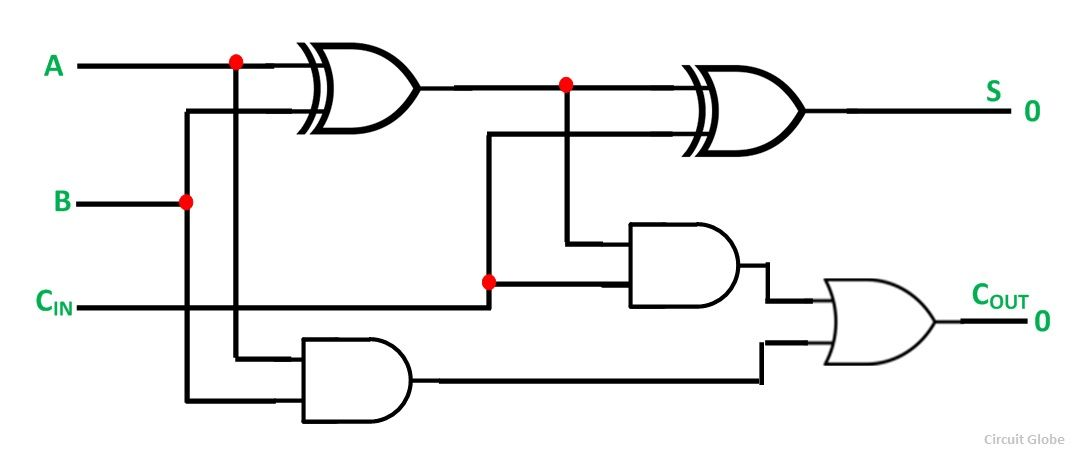
\includegraphics[width=0.5\linewidth]{fulladderfromhalfadder.jpg}
  \caption{A full-adder made from two half-adders.}
  \label{fig:etikett}
\end{figure}

We created an 8-bit ripple carry adder (RCA) by connecting eight full-adders together according to the diagram below. The idea is to simply connect the carry out signal of the first full-adder to the carry in signal of the second one, and so on. The RCA was used in our original design of the ALU but later we replaced it with a carry lookahead adder (CLA).

\begin{figure}[h!]
  \centering
  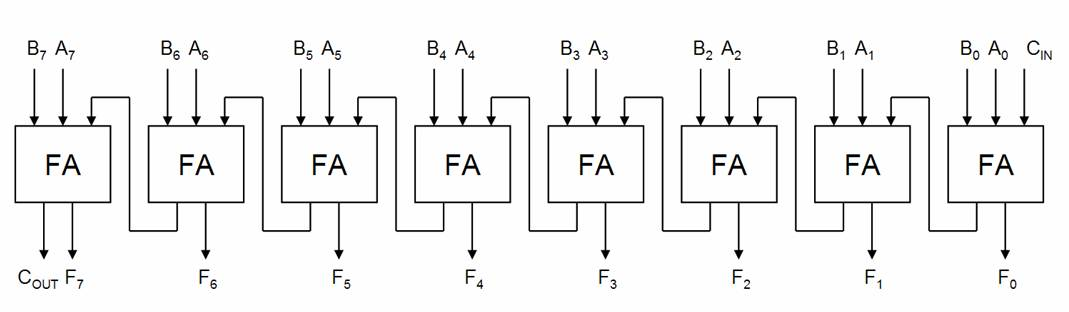
\includegraphics[width=0.9\linewidth]{rca.jpg}
  \caption{A ripple carry adder.}
  \label{fig:etikett}
\end{figure}

The ALU includes a comparator unit which is used to check whether the operands are equal or not. You can implement it by using the structural or dataflow style of VHDL. We decided to do the dataflow implementation because we thought it would be easier and that it would result in a more clean code. In order to check whether the operands are not equal we performed a bitwise XOR on the operands and OR:ed the results. This was used as the resulting NEQ signal. The EQ signal was simply an inversion of the NEQ signal. 

If we were to do this in structural VHDL we would have to create a component which cheked if two certain bits were not equal. We would then have to create eight such components. The input as a whole is equal if all 8 bits are equal, otherwise not.

The operation A minus B is performed by converting B to its 2-complement and then adding it with A. By passing B through 8 XOR gates, each having SUB as its second input, we can form B:s 1-complement when subtracting. We connect SUB to carry-in to form the 2-complement.

\begin{figure}[h!]
  \centering
  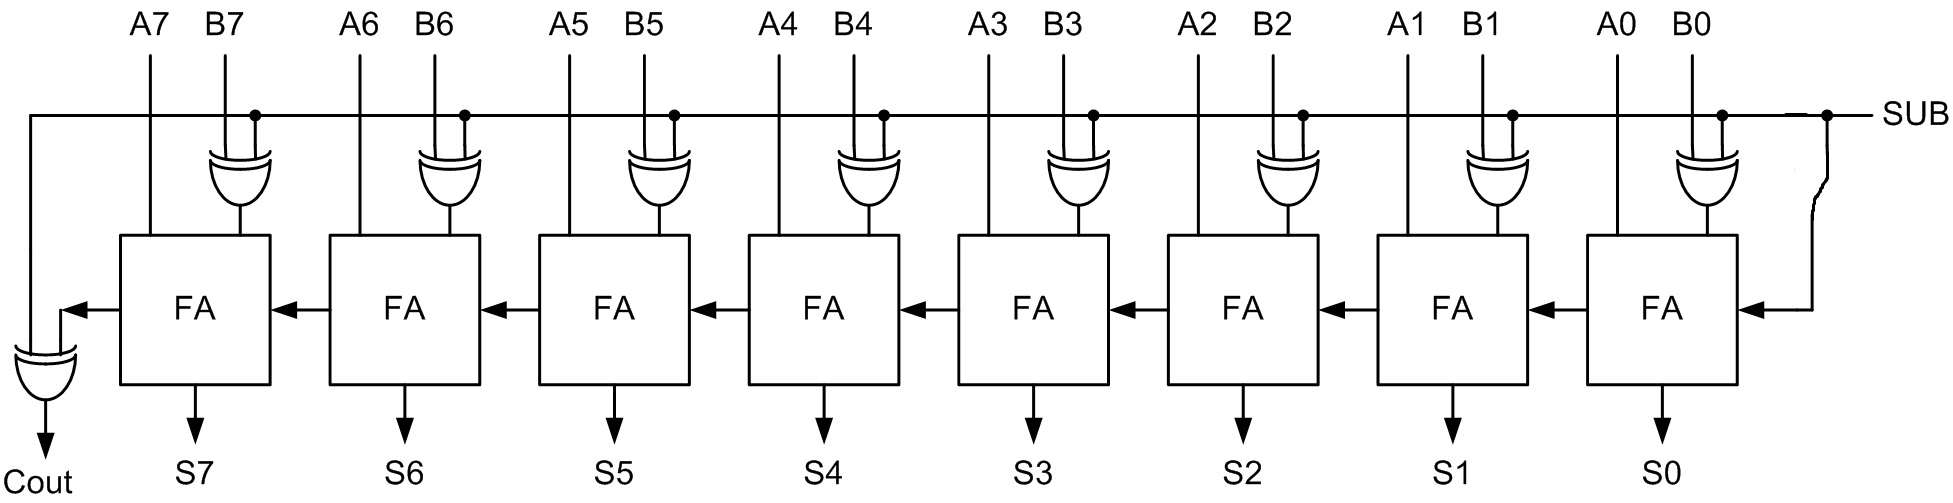
\includegraphics[width=0.90\linewidth]{subtractionlogic.jpg}
  \caption{Logic for performing subtraction with an adder.}
  \label{fig:etikett}
\end{figure}

One thing that we learned was that in VHDL the entity names in a project have to be unique for all references to work properly. 

We also learnt why the critical path for an n-bit RCA is $2n+1$ gates. For every full adder the carry-out depth depends on the inputs ($3$ gates deep) and the carry-in ($2 + $previous depth). The depth is the maximum of these. For the first the depth becomes $3$, for the second $5$ and so on. In other words, for the first adder the inputs are the fartherest away, but for the following it is the carry-in instead. 

\newpage
\subsection{Top-level Design}
(max: 2 pages)
\\\\
Describe what you did in lab 3. In addition, describe how you implemented the bus using the mux and any extra logic or the tri-state buffers. Describe briefly how you implemented the storage elements that are used by the ChAcc processor. Show one snapshot of the simulation waveform where you write something to a memory location and then read from it. Remember to always explain your design choices and mention any assumptions. Finally, make use of figures and tables. 

\textbf{Bus}\\
The bus was implemented with a mux. The 4 indata signals each had 8 bits. Bit 0 from each goes to a 4 to 1 mux, bit 1 from each to another mux and so on, i.e. the signals were muxed bitwise. The muxes are inferred by the tools since we used a \textit{WITH SELECT} statement. The mux select signal was created from a one-hot representation of the 4 control signals. Based on which bit was set, the corresponding mux select signal was created. If 0 or more than 1 bit are set, the bus error signal is set.

We used a multiplexer for the bus since if 2 or more control signals are set, the bus will not take an undefined value, as opossed to a tri-state version. TODO: Why we use the values we do for the bus when 0 or 2+ seleteced. Ask assitants.

\textbf{Datapath}\\
The last step was to connect all components of the datapath as described by figure \ref{fig:datapath}. In the datapath entity we had signals with the same names as on that figure (made it easier to code if the names were the same). We then instatiated all components and connected them together according to the figure. Some components, such as the registers, has different datawidths in different places. But since they were generic it was easy to have multiple versions.

We made a generic implementation of a register by letting a variable hold an integer representing the number of bits the register is able to hold. The vectors for in- and output for the register are adapted after this variable. We implemented our register using behavioral VHDL,i.e using a process statement, since that seemed to result in the simplest and cleanest code. Another reason for using a process statement is that we know that assigning signals values in a process statement result in flip-flops when the code is synthesized.

We also made our implementation of the memory generic. We have two integer variables, one describing the number of address bits (addr\_width) and one describing the number of bits each memory location can hold (data\_width). The number of bits in the input signals for address and data are adjusted after these variables. When instantiating the array representing the memory we use these variables as well. The number of entries in the array are $2^{addr\_width}$ and the size of each entry is data\_width.

\begin{figure}[h!]
  \centering
  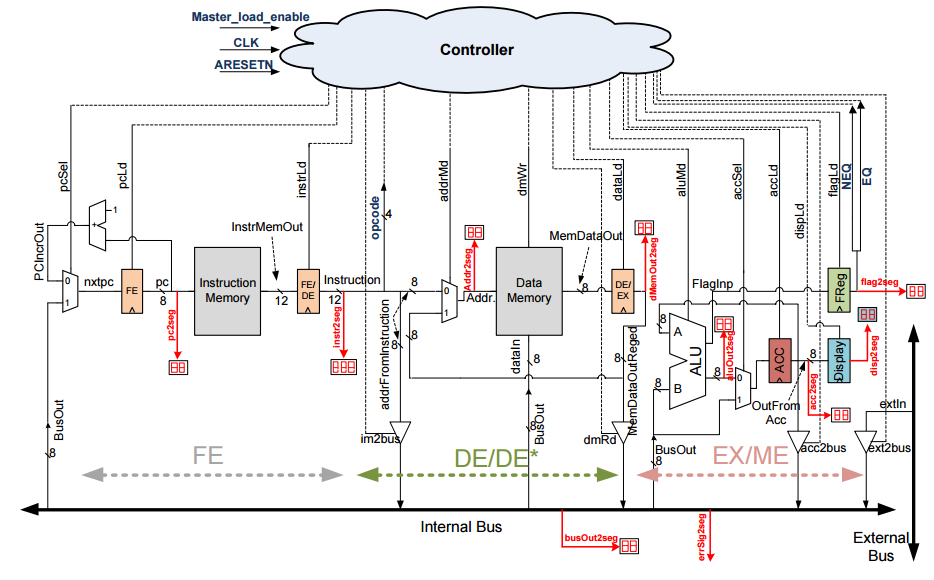
\includegraphics[width=\linewidth]{datapath.png}
  \caption{The datapath of the processor.}
  \label{fig:datapath}
\end{figure} 

\subsection{Controller}
(max: 2 pages)
\\\\
Describe what you did in lab4. More specifically, show the \emph{Finite-state machine} (FSM) of the controller by presenting the diagram you drew. Which design decisions did you make and why? Also include few waveforms, where you show that the controller runs correctly for some particular instructions using the provided testbench. Remember to always explain your design choices and mention any assumptions. Finally, make use of figures and tables. 

\subsection{Processor's Testbench}
(max: 2 pages)
\\\\
Describe what you did in lab5. More specifically, describe how you made the testbench to verify that your processor design was functionally correct. For example, you can specify how you generated inputs to the processor during the testing, how you were reading the expected outputs and how you compare the expected outputs with the actual outputs. Also mention if your processor design was working correctly from the beginning and if not describe how you backtrack the bugs. Remember to always explain your design choices and mention any assumptions. Finally, make use of figures and tables. 

\subsection{ChAcc on Nexys 3 board \emph{(Optional)}}
(max: 2 pages)
\\\\
Describe how you verified the correctness of your FPGA implementation. Note that the code that is executed on the implementation is the same code used for testing in Lab 5. You should compare sequences of values on various signals observed on the seven-segment displays to values seen in Modelsim simulation of the design. Please include in the report the sequence of program counter (PC) and display register values you observed during a successful execution on the FPGA. 

\subsection{Performance, Area and Power Analysis \emph{(Optional)}}
(max: 2 pages)
\\\\
To be announced in the Lab7PM.

\section{Analysis}
(max: 1 page)
\\\\
Summarize your results after performing all the labs (2, 3, 4 and 5).

Mention and discuss interesting findings and observations, as well as difficulties in completing some of the tasks of the four last labs.

After looking at your results, draw conclusions and describe briefly the learning outcome, that is what have you learnt by performing these labs?  

% Appendix
\newpage
\begin{appendix}

\section{Appendix}
(max: 4 pages)
\\\\
In the appendix, you can include extra figures or tables that don't fit in the main body of the lab report. 

\end{appendix}

\end{document}
